The matched finite-gauge family completes 2000 training epochs and 80 scheduled validations at each of $K=32,64,128,256$. Every model reconstructs the same 20 independent random vortical fields with all retained modes and all 1,599,754 fluid points. At $K=256$, the mean relative $L^2$ errors are 0.910006 for Potential-FG and 0.265110 for the same-capacity Laplacian eigenbasis. The corresponding raw-boundary-to-all-basis times are 291.39, 346.78, 451.21, and 665.15 seconds across the four capacities. These measurements include geometry preparation and streamed basis-output I/O.

\begin{figure}[!htb]
\centering
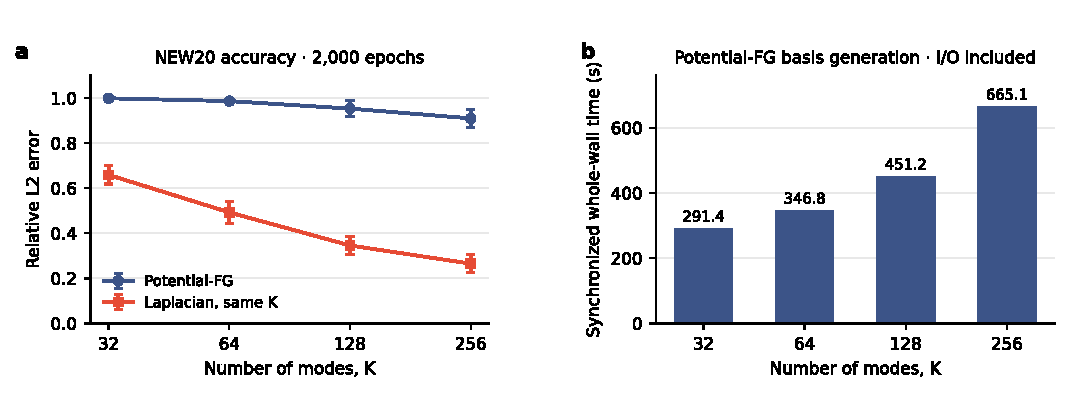
\includegraphics[width=\linewidth]{unified_names_20261021_v1/FG_matched_NEW20_method_names_20261021_v1.pdf}
\caption{\textbf{Matched finite-gauge reconstruction and basis generation.} (a) Relative velocity $L^2$ reconstruction error on 20 independent random vortical fields, using Potential-FG models trained for 2000 epochs and 80 scheduled validations and the same-capacity Laplacian eigenbasis. Error bars show sample standard deviation across the 20 fields. (b) Potential-FG synchronized wall time from raw-boundary JSON parsing and FP64 geometry upload to all 1,599,754 points and all $K$ raw analytic FP64 basis values, including streamed output I/O.}
\label{fig:matched-FG-NEW20}
\end{figure}

\begin{table}[!htb]\centering\small
\caption{Matched Potential-FG reconstruction on the same 20 independent random large-eddy fields, after 2000 epochs and 80 scheduled validations. Relative velocity $L^2$ errors are reported as mean $\pm$ sample standard deviation (\%); all 1,599,754 points and all $K$ modes are retained. The Laplacian entries use the same fields and capacity.}
\label{tab:matched-FG-NEW20-values}
\begin{tabular}{rcc}\toprule
$K$&Matched Potential-FG&Laplacian\\\midrule
32&$99.928\pm0.045$&$65.924\pm4.039$\\
64&$98.690\pm1.315$&$49.278\pm4.782$\\
128&$95.348\pm3.671$&$34.595\pm3.852$\\
256&$91.001\pm4.096$&$26.511\pm3.946$\\
\bottomrule\end{tabular}
\end{table}
